\chapter{Specifikacija programske potpore}
		
	\section{Funkcionalni zahtjevi}
			
			
			\noindent \textbf{Dionici:}
			
			\begin{packed_enum}
				
				\item Banka
				\item Administrator sustava
				\item Službenici banke
				\begin{packed_enum}
					\item Bankari
					\item Službenici za odobravanje kredita građana
				\end{packed_enum}
				\item Klijenti banke
				
			\end{packed_enum}
			
			\noindent \textbf{Aktori i njihovi funkcionalni zahtjevi:}
			
			
			\begin{packed_enum}
				\item  \underbar{Administrator - inicijator}
				
				\begin{packed_enum}
					
					\item Pristup sustavu pomoću korisničkog imena i lozinke
					\item Pregled popisa svih profila i uz njih vezanih korisničkih računa
					\item Dodavanje novih profila u sustav
					\begin{packed_enum}
						\item Unosi ime, prezime, adresu prebivališta, OIB, datum rođenja, e-mail adresu, sliku profila, vrsta korisnika
					\end{packed_enum}
					\item Izmjena podataka profila i mijenjanje razine pristupa korisnicima aplikacije
					\item Brisanje profila korisnika
					\item Dodavanje novog korisničkog računa
					\begin{packed_enum}
						\item Odabir korisničkog imena, sustav generira privremenu lozinku koju je potrebno promijeniti prilikom prve prijave
					\end{packed_enum}
					\item Brisanje korisničkog računa pojedinih profila
					
				\end{packed_enum}
			\eject
				\item  \underbar{Baza podataka - sudionik}
				
				\begin{packed_enum}
					
					\item Sadrži podatke o profilima korisnika sustava
					\begin{packed_enum}
						\item Ime, prezime, adresa, OIB, datum rođenja, e-mail adresa, slika profila, vrsta korisnika
						\item Sve korisničke račune vezane za jedan profil
					\end{packed_enum}
					\item Sadrži podatke o računima klijenata
					\begin{packed_enum}
						\item Broj i stanje tekućeg računa
						\item Broj i stanje žiro računa
						\item Broj i stanje štednog računa
					\end{packed_enum}
					\item Sadrži podatke o karticama klijenata
					\begin{packed_enum}
						\item Broj i vrsta kartice
						\begin{packed_enum}
							\item Debitna kartica - vezana uz račun
							\item Kreditna kartica - nije vezana uz račun
						\end{packed_enum}
						\item Ukoliko je kartica kreditna, sadrži ukupno dugovanje i ukupni odobreni limit po kartici
					\end{packed_enum}
					\item Sadrži podatke o transakcijama među računima klijenata banke
					\item Sadrži podatke o transakcijama po debitnim i kreditnim karticama
					\item Sadrži podatke o kreditima
					\begin{packed_enum}
						\item Iznos, namjena, rok otplate kredita u mjesecima i kamatna stopa
						\item Ukupno preostalo dugovanje (u početku jest iznos uvećan za kamatnu stopu, smanjuje se s otplatom)
					\end{packed_enum}
					
				\end{packed_enum}
				
				\item	\underbar{Bankar - inicijator}
				
				\begin{packed_enum}
					
					\item Inicijalnu prijavu u sustav vrši pomoću korisničkog imena i privremene lozinke dobivene od administratora
					\begin{packed_enum}
						\item Nakon inicijalne prijave obvezan je odmah stvoriti novu lozinku
					\end{packed_enum}
					\item Mogućnost uvida u vlastiti profil
					\begin{packed_enum}
						\item Ime, prezime, adresa, OIB, datum rođenja, e-mail adresa, slika profila
					\end{packed_enum}
					\item Izrada korisničkih profila klijenata banke
					\begin{packed_enum}
						\item Unosi ime, prezime, adresu, OIB, datum rođenja, e-mail adresu, sliku profila klijenta
					\end{packed_enum}
					\item Brisanje korisničkih profila klijenata
					\item Izmjena podataka u korisničkim profilima klijenata
					\item Pretraga profila klijenata pomoću OIB-a klijenta
					\item Otvaranje i zatvaranje tekućih, žiro i štednih računa
					\item Obavljanje transakcija po računima klijenata
					\item Ugovaranje, aktivacija i deaktivacija debitnih i kreditnih kartica
					\item Ugovaranje kredita
					\item Otvaranje korisničkih računa za profile klijenata
					\begin{packed_enum}
						\item Otvaranjem korisničkih računa dobiva prikaz privremenog ključa kojeg korisnik unosi uz svoj OIB kako bi odabrao korisničko ime i lozinku
					\end{packed_enum}
					\item Brisanje korisničkih računa za profile klijenata
					
				\end{packed_enum}
			
				\item	\underbar{Službenik za odobravanje kreditnih zahtjeva - sudionik}
				
				\begin{packed_enum}
					
					\item Inicijalnu prijavu u sustav vrši pomoću korisničkog imena i privremene lozinke dobivene od administratora
					\begin{packed_enum}
						\item Nakon inicijalne prijave obvezan je odmah stvoriti novu lozinku
					\end{packed_enum}
					\item Mogućnost uvida u vlastiti profil
					\begin{packed_enum}
						\item Ime, prezime, adresa, OIB, datum rođenja, e-mail adresa, slika profila
					\end{packed_enum}
					\item Odobrenje i blokiranje kreditnih zahtjeva
					\item Uvid u sve podatke o profilima klijentima čiji zahtjevi za kreditom nisu riješeni
					
				\end{packed_enum}
				
				\item	\underbar{Klijent banke - inicijator}
				
				\begin{packed_enum}
					
					\item Pregledavanje podataka isključivo o vlastitom profilu
					\begin{packed_enum}
						\item Ime, prezime, OIB, adresa, datum rođenja, e-mail adresa, slika profila
						\item Sve ugovorene usluge banke (transakcijski računi, krediti, debitne i kreditne kartice, štedni računi i dr.)
					\end{packed_enum}
					\item Pregledavanje podataka o transakcijama
					\item Prijenos sredstava između vlastitih računa
					\item Prijenos sredstava na račun drugih klijenata
					\item Može ručno izvršiti uplatu kredita ili uplatu na kreditnu karticu kako bi umanjio iznos duga ili kako bi otplatio sveukupno dugovanje
					\item Podnošenje zahtjeva za kreditom
					\begin{packed_enum}
						\item Unosi iznos i namjenu kredita, te rok otplate
					\end{packed_enum}
					\item Podnošenje zahtjeva za kreditnom karticom
					\begin{packed_enum}
						\item Unos vrste kartice (Mastercard, Visa, American Express, Diners, Discover)
					\end{packed_enum}
					
				\end{packed_enum}
				
				\item	\underbar{Neregistrirani korisnik - inicijator}
				
				\begin{packed_enum}
					
					\item Upisuje OIB i jedinstveni ključ dobiven od bankara kako bi se registrirao u sustav
					\item Nakon registracije odabire korisničko ime i lozinku koji će mu služiti za buduće prijave u sustav
					
				\end{packed_enum}
			
			\end{packed_enum}
			
			\eject 
			
			
				
			\subsection{Obrasci uporabe}
				
				\subsubsection{Opis obrazaca uporabe}
				
					\noindent \underbar{\textbf{UC1-Prijava u sustav }}
				\begin{packed_item}
					
					\item \textbf{Glavni sudionik: } Svi korisnici sustava
					\item  \textbf{Cilj:} Dobiti pristup sustavu
					\item  \textbf{Sudionici:} Baza podataka
					\item  \textbf{Preduvjet:} Korisnik ima korisnički račun
					\item  \textbf{Opis osnovnog tijeka:}
					
					\item[] \begin{packed_enum}
						
						\item Korisnik sustava unosi korisničko ime i lozinku
						\item Potvrda o ispravnosti korisničkih podataka
						\item Korisnik sustava dobiva pristup sustavu
						
					\end{packed_enum}
					
					\item  \textbf{Opis mogućih odstupanja:}
					
					\item[] \begin{packed_item}
						
						\item[2.a] Unos neispravnih podataka
						\item[] \begin{packed_enum}
							
							\item Ispis odgovarajuće poruke upozorenja 
							
							
						\end{packed_enum}
						
						
					\end{packed_item}
				\end{packed_item}
			
			
				\noindent \underbar{\textbf{UC2-Pregled profila svih korisnika sustava }}
				\begin{packed_item}
					
					\item \textbf{Glavni sudionik:} Administrator
					\item  \textbf{Cilj:} Pregledati registrirane korisnike i njihove osobne podatke
					\item  \textbf{Sudionici:} Baza podataka
					\item  \textbf{Preduvjet:} : Korisnik je registriran i dodijeljena su mu prava administratora
					\item  \textbf{Opis osnovnog tijeka:}
					
					\item[] \begin{packed_enum}
						
						\item Administrator odabire opciju pregledavanja korisnika
						\item Prikazuje se lista svih profila korisnika
						
					\end{packed_enum}
					
				\end{packed_item}
				
				
				
				
				
		   	\noindent \underbar{\textbf{UC3-Dodavanje novih profila u sustav }}
				\begin{packed_item}
						
						\item \textbf{Glavni sudionik: }Administrator
						\item  \textbf{Cilj:} Dodati profil u sustav
						\item  \textbf{Sudionici:} Baza podataka
						\item  \textbf{Preduvjet:} Profil se ne nalazi u bazi podataka
						\item  \textbf{Opis osnovnog tijeka:}
						
						\item[] \begin{packed_enum}
							
							\item Administrator unosi potrebne osobne podatke
							\begin{packed_enum}
								\item Ime, prezime, adresa, OIB, datum rodenja, e-mail adresa, slika profila, vrsta korisnika (razina pristupa sustavu)
							\end{packed_enum}
							\item Podaci se unose u bazu podataka
							\item Stvoren je novi profil
							
						\end{packed_enum}
						
						\item  \textbf{Opis mogućih odstupanja:}
						
						\item[] \begin{packed_item}
							
							\item[1.a] Unos neispravnih podataka (krivi OIB, profil s tim OIB-om ime već postoji i dr.)
							\item[] \begin{packed_enum}
								
								\item Ispis odgovarajuće poruke upozorenja
								
							\end{packed_enum}
							
						\end{packed_item}
					\end{packed_item}
				
				
				\noindent \underbar{\textbf{UC4-Izmjena podataka profila korisnika  }}
				\begin{packed_item}
					
					\item \textbf{Glavni sudionik: }Administrator
					\item  \textbf{Cilj:} Urediti i izmijeniti podatke profila
					\item  \textbf{Sudionici:} Baza podataka
					\item  \textbf{Preduvjet:} Korisnik je prijavljen u sustav kao administrator
					\item  \textbf{Opis osnovnog tijeka:}
					
					\item[] \begin{packed_enum}
						
						\item Administrator otvara željeni profil iz popisa svih korisnika
						\item Administrator odabire opciju uređivanja profila
						\item Administrator izmjenjuje podatke korisnika i sprema ih u bazu podataka 
						
					\end{packed_enum}
					
					
				\end{packed_item}
			
			
			\noindent \underbar{\textbf{UC5-Brisanje profila korisnika }}
			\begin{packed_item}
				
				\item \textbf{Glavni sudionik: }Administrator
				\item  \textbf{Cilj:} Obrisati korisnika
				\item  \textbf{Sudionici:} Baza podataka
				\item  \textbf{Preduvjet:} Korisnik je prijavljen u sustav kao administrator
				\item  \textbf{Opis osnovnog tijeka:}
				
				\item[] \begin{packed_enum}
					
					\item Administrator otvara željeni profil iz popisa svih korisnika
					\item Administrator odabire opciju brisanja profila
					\item Uklanja se korisnik i njegovi podaci iz baze podataka
					
				\end{packed_enum}
				
				
			\end{packed_item}
				
							
			
			\noindent \underbar{\textbf{UC6 - Promjena razine pristupa profila }}
			\begin{packed_item}
				
				\item \textbf{Glavni sudionik: }Administrator
				\item  \textbf{Cilj:} Promijeniti razinu pristupa korisnika sustavu (administrator, bankar, službenik za odobravanje kreditnih zahtjeva klijenata, klijent banke)
				\item  \textbf{Sudionici:} Baza podataka
				\item  \textbf{Preduvjet:} Korisnik je prijavljen u sustav kao administrator
				\item  \textbf{Opis osnovnog tijeka:}
				
				\item[] \begin{packed_enum}
					
					\item Administrator odabire željenog korisnika s popisa profila
					\item Izmijeni razinu pristupa korisnika
					
					
				\end{packed_enum}
				
			\end{packed_item}
			
			\noindent \underbar{\textbf{UC7 - Dodavanje novog korisničkog računa }}
			\begin{packed_item}
				
				\item \textbf{Glavni sudionik: }Administrator
				\item  \textbf{Cilj:} Dozvoliti pristup sustavu nekom korisniku
				\item  \textbf{Sudionici:} Baza podataka
				\item  \textbf{Preduvjet:} Korisnik je prijavljen u sustav kao administrator, postoji profil korisnika kome želimo dodati korisnički račun
				\item  \textbf{Opis osnovnog tijeka:}
				
				\item[] \begin{packed_enum}
					
					\item Administrator otvara željeni profil iz popisa svih korisnika
					\item Administrator odabire opciju dodavanja korisničkog računa
					\item Administrator odabire korisničko ime i privremenu lozinku koja se mora promijeniti prilikom prve prijave s tim vjerodajnicama
					
					
				\end{packed_enum}
			
				\item  \textbf{Opis mogućih odstupanja:}
				
				\item[] \begin{packed_item}
					
					\item[3.1] Unos već postojećeg korisničkog ime
					\item[] \begin{packed_enum}
						
						\item Ispis odgovarajuće poruke upozorenja
						\item Korisnički račun ne dodaje se u sustav
						
					\end{packed_enum}
					
				\end{packed_item}
				
			\end{packed_item}
		
			
			\noindent \underbar{\textbf{UC8 - Brisanje korisničkog računa }}
			\begin{packed_item}
				
				\item \textbf{Glavni sudionik: }Administrator
				\item  \textbf{Cilj:} Onemogućiti pristup sustavu nekom korisniku
				\item  \textbf{Sudionici:} Baza podataka
				\item  \textbf{Preduvjet:} Korisnik je prijavljen u sustav kao administrator, postoji profil korisnika koji ima korisnički račun vezan za sebe
				\item  \textbf{Opis osnovnog tijeka:}
				
				\item[] \begin{packed_enum}
					
					\item Administrator otvara željeni profil iz popisa svih korisnika
					\item U popisu korisničkih računa vezanih za odabrani profil, odabere onog kojeg želi obrisati
					\item Administrator potvrđuje opciju uklanjanja korisničkog računa
										
				\end{packed_enum}
				
			\end{packed_item}
		
			
			\noindent \underbar{\textbf{UC9 - Inicijalna prijava bankara}}
			\begin{packed_item}
				
				\item \textbf{Glavni sudionik: }Bankar
				\item  \textbf{Cilj:} Aktivirati korisnički račun za pristup sustavu
				\item  \textbf{Sudionici:} Baza podataka
				\item  \textbf{Preduvjet:} Dobivena privremena lozinka i korisničko ime od administratora
				\item  \textbf{Opis osnovnog tijeka:}
				
				\item[] \begin{packed_enum}
					
					\item  Bankar odabire opciju za prijavu
					\item  Bankar unosi korisničko ime i privremenu lozinku dobivene od administratora
					\item  Bankar mijenja privremenu lozinku 
					\item  U bazu podataka se pohrani promjena 
				\end{packed_enum}
				
				\item  \textbf{Opis mogućih odstupanja:}
				
				\item[] \begin{packed_enum}
					
					\item[2.a] Upisana kriva kombinacija korisničkog imena i privremen lozinke
					\item[] \begin{packed_enum}
						
						\item Sustav obavještava korisnika o neuspjelom upisu 
						
					\end{packed_enum}
					
					\item[3.a] Korisnikova nova lozinka identična je privremenoj
					\item[] \begin{packed_enum}
						
						\item Sustav obavještava korisnika o obaveznom mijenjanju privremene lozinke
						
						
						\end{packed_enum}
					\end{packed_enum}
			\end{packed_item}
		
		
			\noindent \underbar{\textbf{UC10 - Uvid u vlastite osobne podatke }}
			\begin{packed_item}
				
				\item \textbf{Glavni sudionik: }Bankar
				\item  \textbf{Cilj:} Pregledati osobne podatke
				\item  \textbf{Sudionici:} Baza podatak
				\item  \textbf{Preduvjet:} Korisnik je prijavljen u sustav i dodijeljena su mu prava bankara 
				\item  \textbf{Opis osnovnog tijeka:}
				
				\item[] \begin{packed_enum}
					\item  Korisnik odabire opciju ”Osobni podatci"
					\item  Aplikacija prikazuje osobne podatke : ime, prezime, adresu, OIB, datum rođenja, e-mail adresu i sliku profila korisnika
				\end{packed_enum}
				
			\end{packed_item}
            		
          
          
            \noindent \underbar{\textbf{UC11 - Izrada novog korisničkog profila klijenta banke }}
            \begin{packed_item}
                
                  \item \textbf{Glavni sudionik: }Bankar
                  \item  \textbf{Cilj:} Dodati novi korisnički profil
                  \item  \textbf{Sudionici:} Baza podataka
                  \item  \textbf{Preduvjet:} Korisnik je prijavljen u sustav i dodijeljena su mu prava bankara te klijent nema korisnički profil
                  \item  \textbf{Opis osnovnog tijeka:}
                  
                  \item[] \begin{packed_enum}
                
                    \item  Bankar odabire opciju izrade novog korisničkog profila klijenta
                    \item  Otvara se prozor za upis osobnih podataka klijenta
                    \item  Bankar upiše ime, prezime, adresu, OIB, datum rođenja, e-mail adresu, sliku profila i potvrdi upis
                    \item  U bazu podataka se pohrani promjena                              
                  \end{packed_enum}
                  
                \end{packed_item}
            
                
                
                \noindent \underbar{\textbf{UC12 - Brisanje korisničkog profila klijenta }}
                \begin{packed_item}
                
                  \item \textbf{Glavni sudionik: }Bankar
                  \item  \textbf{Cilj:} Obrisati korisnički profil 
                  \item  \textbf{Sudionici:} Baza podataka
                  \item  \textbf{Preduvjet:} Korisnik je prijavljen u sustav i dodijeljena su mu prava bankara te klijent ima korisnički profil
                  \item  \textbf{Opis osnovnog tijeka:}
              
              \item[] \begin{packed_enum}
                
                    \item  Bankar u tražilicu upisuje OIB klijenta
                    \item  Otvara se profil traženog klijenta sa svim njegovim podacima i opcijom "obriši profil"
                    \item  Bankar odabere opciju "obriši profil" i potvrđuje odabir
                    \item  U bazu podataka se pohrani promjena (briše se i profil i svi korisnički računi klijenta vezani uz profil)
                  \end{packed_enum}
                  
                  \item  \textbf{Opis mogućih odstupanja:}
                  
                  \item[] \begin{packed_enum}
                
                    \item[1.a] Upisan nepostojeći OIB
                    \item[] \begin{packed_enum}
                      
                      \item Sustav obavještava bankara o neuspjelom upisu OIB-a 
                    
                  \end{packed_enum}
                \end{packed_enum}
            \end{packed_item}
        
                
                \noindent \underbar{\textbf{UC13 - Ažuriranje korisničkog profila klijenta}}
                \begin{packed_item}
                
                  \item \textbf{Glavni sudionik: }Bankar
                  \item  \textbf{Cilj:} Izmijeniti korisnički profil klijenta 
                  \item  \textbf{Sudionici:} Baza podataka
                  \item  \textbf{Preduvjet:} Korisnik je prijavljen u sustav i dodijeljena su mu prava bankara te klijent ima korisnički profil
                  \item  \textbf{Opis osnovnog tijeka:}
                  
                  \item[] \begin{packed_enum}
                
                    \item  Bankar u tražilicu upisuje OIB klijenta
                    \item  Bankar pronalazi željenog korisnika
                    \item  Bankar mijenja podatke u profilu klijenta
                    \item  Bankar odabire opciju "Spremi"
                    \item  U bazu podataka se pohrani promjena                     
                    \item  Korisnik vidi promjene korisničkog profila u aplikaciji 
                  \end{packed_enum}
                  
                  \item  \textbf{Opis mogućih odstupanja:}
                  
                  \item[] \begin{packed_item}
                  	
                  	 \item[1.a] Upisan nepostojeći OIB
                  	\item[] \begin{packed_enum}
                  		
                  		\item Sustav obavještava bankara o neuspjelom upisu OIB-a 
                  		
                  		
                  	\end{packed_enum}
                
                    \item[3.a] Bankar unosi novi nevažeći OIB
                    \item[] \begin{packed_enum}
                      
                      \item Sustav obavještava korisnika da nije spremio podatke
                      
                    \end{packed_enum}
                  
                \end{packed_item}
            \end{packed_item}
        
        
                
               \noindent \underbar{\textbf{UC14 - Otvaranje računa}}
                \begin{packed_item}
            
                  \item \textbf{Glavni sudionik: }Bankar
                  \item  \textbf{Cilj:} Otvoriti račun klijentu
                  \item  \textbf{Sudionici:} Baza podataka
                  \item  \textbf{Preduvjet:} Korisnik je prijavljen u sustav i dodijeljena su mu prava bankara te klijent ima korisnički profil
                  \item  \textbf{Opis osnovnog tijeka:}
                  
                  \item[] \begin{packed_enum}
                
                	\item Bankar u tražilicu upisuje OIB klijenta
                	\item Bankar pronalazi željenog korisnika
                    \item Bankar odabire opciju "Izrada računa" 
                    \item Odabire iz padajućeg izbornika tekući, žiro ili štedni
                    \item Odabire opciju "Otvori"
                    \item Promjene spremljene u bazu podataka                 
                    \item Klijentu se omogućuje prikaz računa u aplikaciji - broj računa i iznos sredstava na računu
                   \end{packed_enum}
                  
                \end{packed_item}
                
                
                \noindent \underbar{\textbf{UC15 - Zatvaranje računa}}
                \begin{packed_item}
                
                  \item \textbf{Glavni sudionik: }Bankar
                  \item  \textbf{Cilj:} Zatvoriti račun klijentu
                  \item  \textbf{Sudionici:} Baza podataka
                  \item  \textbf{Preduvjet:} Korisnik je prijavljen u sustav i dodijeljena su mu prava bankara te klijent ima korisnički profil i otvoren transakcijski račun
                  \item  \textbf{Opis osnovnog tijeka:}
                  
                  \item[] \begin{packed_enum}
                
                	\item Bankar u tražilicu upisuje OIB klijenta
                	\item Bankar pronalazi željenog korisnika
                    \item Bankar pored željenog računa odabire opciju "Zatvaranja računa"
                    \item Odabire opciju "Zatvori" (potvrđuje odabrano)                  
                    \item U bazu podataka se pohrani promjena
                  \end{packed_enum}
                 
                \end{packed_item}
            
	            \noindent \underbar{\textbf{UC16 - Obavljanje transkacija po računima klijenata}}
	            \begin{packed_item}
	            	
	            	\item \textbf{Glavni sudionik: }Bankar
	            	\item  \textbf{Cilj:} Obaviti transakciju po računu klijenata
	            	\item  \textbf{Sudionici:} Baza podataka
	            	\item  \textbf{Preduvjet:} Korisnik je prijavljen u sustav i dodijeljena su mu prava bankara te klijent ima korisnički profil i otvoren transakcijski račun
	            	\item  \textbf{Opis osnovnog tijeka:}
	            	
	            	\item[] \begin{packed_enum}
	            		
	            		\item Bankar u tražilicu upisuje OIB klijenta
	            		\item Bankar pronalazi željenog korisnika
	            		\item Bankar odabire opciju "Transfer"
	            		\item Otvara se novi prozor u kojem je za račun terećenja padajući izbornik - mogućnost odabira samo računa trenutnog klijenta
	            		\item Otvara se polje za upis računa odobrenja i bankar upisuje bilo čiji broj računa i iznos transfera te poziv na broj transakcije
	            		\item U bazu podataka se pohrani promjena 
	            	\end{packed_enum}
	            	
	            	\item  \textbf{Opis mogućih odstupanja:} 
	            	
	            	\item[] \begin{packed_item}
	            		
	            		\item[3.a] Upisan nepostojeći račun  odobrenja ili ako je iznos transfera veći nego što klijent ima na računu terećenja
	            		\item[] \begin{packed_enum}
	            			
	            			\item Sustav obavještava bankara o neuspjelom upisu 
	            			
	            		\end{packed_enum}
	            		
	            	\end{packed_item}
	            \end{packed_item}
                            
                
                \noindent \underbar{\textbf{UC17 -Ugovaranje debitne kartice}}
                \begin{packed_item}
                
                  \item \textbf{Glavni sudionik: }Bankar
                  \item  \textbf{Cilj:} Ugovoriti debitnu karticu klijentu
                  \item  \textbf{Sudionici:} Baza podataka
                  \item  \textbf{Preduvjet:} Korisnik je prijavljen u sustav i dodijeljena su mu prava bankara
                  \item  \textbf{Opis osnovnog tijeka:}
                  
                  \item[] \begin{packed_enum}
                
                	\item Bankar u tražilicu upisuje OIB klijenta
                	\item Bankar pronalazi željenog korisnika
                    \item Bankar odabire opciju "Dodaj karticu" pored željenog transakcijskog računa za račun koji nema debitnu karticu
                    \item Promjene se spremaju u bazu podataka
                    \item Dodaje se mogućnost uvida u broj kartice i račun uz koji je vezana preko korisničkog profila klijenta            
                  \end{packed_enum}
                  
                  \item  \textbf{Opis mogućih odstupanja:}
                  
                  \item[] \begin{packed_item}
                
                        \item[1.a] Upisan nepostojeći OIB klijenta
                    \item[] \begin{packed_enum}
                      
                      \item Sustav obavještava bankara o neuspjelom upisu OIB-a
                      
                    \end{packed_enum}
                    
                  \end{packed_item}
                \end{packed_item}
                
                
                \noindent \underbar{\textbf{UC18 -Ugovaranje kreditnih kartica}}
                \begin{packed_item}
                
                  \item \textbf{Glavni sudionik: }Bankar
                  \item  \textbf{Cilj:} Ugovoriti kreditnu karticu klijentu
                  \item  \textbf{Sudionici:} Baza podataka
                  \item  \textbf{Preduvjet:} Korisnik je prijavljen u sustav i dodijeljena su mu prava bankara
                  \item  \textbf{Opis osnovnog tijeka:}
                  
                  \item[] \begin{packed_enum}
                
                	\item Bankar u tražilicu upisuje OIB klijenta
                	\item Bankar pronalazi željenog korisnika
                    \item Bankar odabire opciju "Ugovaranje kreditne kartice"
                    \item Bankar bira vrstu kreditne kartice (Visa, MasterCard, Diners, Amercan Express, Discover i dr.)
                    \item Promjene se spremaju u bazu podataka
                    \item Zahtjev odlazi službeniku za odobravanje kreditnih zahtjeva na odobravanje
                  \end{packed_enum}
                  
                  \item  \textbf{Opis mogućih odstupanja:}
                  
                  \item[] \begin{packed_item}
                
                    \item[1.a] Upisan nepostojeći OIB klijenta
                    \item[] \begin{packed_enum}
                      
                      \item Sustav obavještava bankara o neuspjelom upisu OIB-a
                      
                    \end{packed_enum}
                    
                  \end{packed_item}
                \end{packed_item}
            
            
            	\noindent \underbar{\textbf{UC19 - Aktiviranje kartica klijenta}}
            	\begin{packed_item}
            		
            		\item \textbf{Glavni sudionik: }Bankar
            		\item  \textbf{Cilj:} Aktivirati karticu klijentu
            		\item  \textbf{Sudionici:} Baza podataka
            		\item  \textbf{Preduvjet:} Korisnik je prijavljen u sustav i dodijeljena su mu prava bankara te je klijent zatražio aktivaciju kartice
            		\item  \textbf{Opis osnovnog tijeka:}
            		
            		\item[] \begin{packed_enum}
            			
            			\item Bankar u tražilicu upisuje OIB klijenta
            			\item Bankar pronalazi željenog korisnika
            			\item Bankar u popisu kartica odabire opciju "Aktivacija kartice" uz željenu karticu
            			\item Bankar odabire opciju "Potvrdi"
            			\item U bazu podataka se pohrani promjena 
            			\item Omogućeno je provođenje transakcija karticom
            		\end{packed_enum}
            		
            		\item  \textbf{Opis mogućih odstupanja:} 
            		
            		\item[] \begin{packed_item}
            			
            			\item[1.a] Upisan nepostojeći OIB klijenta
            			\item[] \begin{packed_enum}
            				
            				\item Sustav obavještava bankara o neuspjelom upisu OIB-a
            				
            			\end{packed_enum}
            			
            		\end{packed_item}
            	\end{packed_item}
                
                
                \noindent \underbar{\textbf{UC20 - Deaktiviranje kartica klijenta}}
                \begin{packed_item}
                	
                	\item \textbf{Glavni sudionik: }Bankar
                	\item  \textbf{Cilj:} Deaktivirati karticu klijentu
                	\item  \textbf{Sudionici:} Baza podataka
                	\item  \textbf{Preduvjet:} Korisnik je prijavljen u sustav i dodijeljena su mu prava bankara te je klijent zatražio deaktivaciju kartice
                	\item  \textbf{Opis osnovnog tijeka:}
                	
                	\item[] \begin{packed_enum}
                		
                		\item Bankar u tražilicu upisuje OIB klijenta
                		\item Bankar pronalazi željenog korisnika
                		\item Bankar u popisu kartica odabire opciju "Dektivacija kartice" uz željenu karticu
                		\item Bankar odabire opciju "Potvrdi"
                		\item U bazu podataka se pohrani promjena 
                		\item Onemogućeno je provođenje transakcija karticom
                	\end{packed_enum}
                	
                	\item  \textbf{Opis mogućih odstupanja:} 
                	
                	\item[] \begin{packed_item}
                		
                		\item[1.a] Upisan nepostojeći OIB klijenta
                		\item[] \begin{packed_enum}
                			
                			\item Sustav obavještava bankara o neuspjelom upisu OIB-a
                			
                		\end{packed_enum}
                		
                	\end{packed_item}
                \end{packed_item}
                
                
                
                 \noindent \underbar{\textbf{UC21 - Ugovaranje kredita}}
                \begin{packed_item}
                	
                	\item \textbf{Glavni sudionik: }Bankar
                	\item  \textbf{Cilj:} ugovoriti kredit klijentu
                	\item  \textbf{Sudionici:} Baza podataka
                	\item  \textbf{Preduvjet:} Korisnik je prijavljen u sustav i dodijeljena su mu prava bankara te je klijent zatražio ugovaranje kredita
                	\item  \textbf{Opis osnovnog tijeka:}
                	
                	\item[] \begin{packed_enum}
                		
                		\item Bankar u tražilicu upisuje OIB klijenta
                		\item Bankar pronalazi željenog korisnika
                		\item Bankar odabire opciju "Ugovaranje kredita"
                		\item Unos odgovarajućih podataka
                		\begin{packed_enum}
                			\item Iznos, namjena kredita, rok otplate kredita u mjesecima
                			\item Kamatna stopa određena je namjenom kredita
                		\end{packed_enum}
                		\item U bazu podataka se pohrani promjena 
                		\item Klijent se dodaje na listu koja se šalje službeniku za odobravanje kredita
                	\end{packed_enum}
                	
                	\item  \textbf{Opis mogućih odstupanja:} 
                	
                	\item[] \begin{packed_item}
                		
                		\item[1.a] Upisan nepostojeći OIB klijenta
                		\item[] \begin{packed_enum}
                			
                			\item Sustav obavještava bankara o neuspjelom upisu OIB-a
                			
                		\end{packed_enum}
                		
                	\end{packed_item}
                \end{packed_item}
            
            	\noindent \underbar{\textbf{UC22 - Otvaranje korisničkih računa za profile klijenata}}
            	\begin{packed_item}
            		
            		\item \textbf{Glavni sudionik: }Bankar
            		\item  \textbf{Cilj:} Omogućiti klijentu pristup sustavu
            		\item  \textbf{Sudionici:} Baza podataka
            		\item  \textbf{Preduvjet:} Korisnik je prijavljen u sustav i dodijeljena su mu prava bankara te je klijent zatražio otvaranje korisničkog računa
            		\item  \textbf{Opis osnovnog tijeka:}
            		
            		\item[] \begin{packed_enum}
            			
            			\item Bankar u tražilicu upisuje OIB klijenta
            			\item Bankar pronalazi željenog korisnika
            			\item Bankar odabire opciju "Dodaj korisnički račun"
            			\item Bankar dobiva privremeni ključ za klijenta
            		\end{packed_enum}
            		
            		\item  \textbf{Opis mogućih odstupanja:} 
            		
            		\item[] \begin{packed_item}
            			
            			\item[1.a] Upisan nepostojeći OIB klijenta
            			\item[] \begin{packed_enum}
            				
            				\item Sustav obavještava bankara o neuspjelom upisu OIB-a
            				
            			\end{packed_enum}
            			
            		\end{packed_item}
            	\end{packed_item}
            
            	\noindent \underbar{\textbf{UC23 - Zatvaranje korisničkih računa za profile klijenata}}
            	\begin{packed_item}
            		
            		\item \textbf{Glavni sudionik: }Bankar
            		\item  \textbf{Cilj:} Onemogućiti klijentu pristup sustavu
            		\item  \textbf{Sudionici:} Baza podataka
            		\item  \textbf{Preduvjet:} Korisnik je prijavljen u sustav i dodijeljena su mu prava bankara te je klijent zatražio zatvaranje korisničkog računa
            		\item  \textbf{Opis osnovnog tijeka:}
            		
            		\item[] \begin{packed_enum}
            			
            			\item Bankar u tražilicu upisuje OIB klijenta
            			\item Bankar pronalazi željenog korisnika
            			\item Odabire opciju "obriši korisnički račun" pored željenog računa s popisa svih vezanih računa
            			\item U bazu podataka se pohrani promjena
            		\end{packed_enum}
            		
            		\item  \textbf{Opis mogućih odstupanja:} 
            		
            		\item[] \begin{packed_item}
            			
            			\item[1.a] Upisan nepostojeći OIB klijenta
            			\item[] \begin{packed_enum}
            				
            				\item Sustav obavještava bankara o neuspjelom upisu OIB-a
            				
            			\end{packed_enum}
            			
            		\end{packed_item}
            	\end{packed_item}            
            
                \noindent \underbar{\textbf{UC24 - Odobrenje kreditnih zahtjeva}}
                \begin{packed_item}
                	
                	\item \textbf{Glavni sudionik: } Službenik za odobravanje kredita
                	\item  \textbf{Cilj:} Odobriti zahtjev za kredit klijentu
                	\item  \textbf{Sudionici:} Baza podataka
                	\item  \textbf{Preduvjet:} Korisnik je registriran i dodijeljena su mu prava službenika za odobravanje kreditnih zahtjeva 
                	\item  \textbf{Opis osnovnog tijeka:}
                	
                	\item[] \begin{packed_enum}
                		
                		\item Preuzimanje liste zahtjeva za kredit
                		\item Odabir jednog od zahtjeva
                		\begin{packed_enum}
                			\item Ako je zahtjev za kreditnom karticom, službenik dodatno unosi odobreni limit po kartici te kamatnu stopu na iskorišteni dio limita
                		\end{packed_enum}
                		\item Odabir opcije "odobri"
                		\item Spremanje promjena u bazu podataka
                		\item Odluka o odobrenju postaje vidljiva korisniku unutar aplikacije
                		
                	\end{packed_enum}
                \end{packed_item}
            
            
                \noindent \underbar{\textbf{UC25 - Blokiranje kreditnih zahtjeva}}
                \begin{packed_item}
                
                  \item \textbf{Glavni sudionik: } Službenik za odobravanje kredita
                  \item  \textbf{Cilj:} Blokirati zahtjev za kredit klijentu
                  \item  \textbf{Sudionici:} Baza podataka
                  \item  \textbf{Preduvjet:} Korisnik je registriran i dodijeljena su mu prava službenika za odobravanje kreditnih zahtjeva 
                  \item  \textbf{Opis osnovnog tijeka:}
                  
                  \item[] \begin{packed_enum}
                
                    \item Preuzimanje liste zahtjeva za kredit
                    \item Odabir jednog od zahtjeva 
                    \item Odabir opcije "blokiraj"
                    \item Spremanje promjena u bazu podataka
                    \item Odluka o blokiranju postaje vidljiva korisniku unutar aplikacije
                    
                      \end{packed_enum}
                    \end{packed_item}
                
            
                 \noindent \underbar{\textbf{UC26 - Uvid u podatke o klijentima}}
                    \begin{packed_item}
                    
                      \item \textbf{Glavni sudionik: } Službenik za odobravanje kredita
                      \item  \textbf{Cilj:} Uvid u profil klijenta za kojeg djelatnik obrađuje zahtjev
                      \item  \textbf{Sudionici:} Baza podataka
                      \item  \textbf{Preduvjet:} Korisnik je registriran i dodijeljena su mu prava službenika za odobravanje kreditnih zahtjeva te je klijent podnio zahtjev za kredit
                      \item  \textbf{Opis osnovnog tijeka:}
                      
                      \item[] \begin{packed_enum}
                    
                    \item S liste zahtjeva za kredit, službenik bira klijenta čije osobne podatke želi pregledati u svrhu odobravanja kredita
                    \item Prikazuju se svi dostupni podaci u profilu klijenta: ime, prezime, adresa, OIB, datum rođenja, e-mail adresa, slika profila, podaci o računima: broj i stanje računa, podaci o kreditnim karticama, podaci o ugovorenim kreditima: iznos, trajanje otplate, podaci o kreditnim karticama i ostalo
                    
                    
                  \end{packed_enum}
                \end{packed_item}
            
	            \noindent \underbar{\textbf{UC27 - Pregled podataka o vlastitom profilu }}
	            \begin{packed_item}
	            	
	            	\item \textbf{Glavni sudionik: } Službenik za odobravanje kredita
	            	\item  \textbf{Cilj:} Pregledati podatke na vlastitom profilu
	            	\item  \textbf{Sudionici:} Baza podataka
	            	\item  \textbf{Preduvjet:} Korisnik sustava je prijavljen
	            	\item  \textbf{Opis osnovnog tijeka:}
	            	
	            	\item[] \begin{packed_enum}
	            		
	            		\item Korisnik sustava odabire opciju pregleda osobnih podataka
	            		\item Aplikacija prikazuje osobne podatke korisnika
	            		
	            	\end{packed_enum}
	            	
	            \end{packed_item}
        			
        		  \noindent \underbar{\textbf{UC28 - Pregled podataka o vlastitom profilu }}
        			\begin{packed_item}
        				
        				\item \textbf{Glavni sudionik: }Klijent
        				\item  \textbf{Cilj:} Pregledati podatke na vlastitom profilu
        				\item  \textbf{Sudionici:} Baza podataka
        				\item  \textbf{Preduvjet:} Klijent je prijavljen
        				\item  \textbf{Opis osnovnog tijeka:}
        				
        				\item[] \begin{packed_enum}
        					
        					\item Korisnik odabire opciju pregleda osobnih podataka
        					\item Aplikacija prikazuje sve podatke korisnika
        					\begin{packed_enum}
        						\item Osobne podatke (ime, prezime, adresa prebivališta, OIB, datum rođenja, e-mail adresa, slika profila)
        						\item Podatke o računima (tekućim, žiro i štednim) : brojevi računa i stanje na računu
        						\item Podatke o karticama (debitnim i kreditnim) : broj kartice, broj računa za koji je kartica vezana (debitna), odobren i iskorišten limit kartice (kreditna)
        						\item Podatke o kreditima (Iznos kredita, kamatna stopa, rok otplate, datum ugovaranja, preostalo dugovanje)
        					\end{packed_enum}
    					
    				\end{packed_enum}
    				
    			\end{packed_item}
    			
    			\noindent \underbar{\textbf{UC29 - Pregled podataka o transakcijama }}
    			\begin{packed_item}
    				
    				\item \textbf{Glavni sudionik: }Klijent
    				\item  \textbf{Cilj:} Pregledati podatke o transakcijama
    				\item  \textbf{Sudionici:} Baza podataka
    				\item  \textbf{Preduvjet:} Klijent je prijavljen
    				\item  \textbf{Opis osnovnog tijeka:}
    				
    				\item[] \begin{packed_enum}
    					
    					\item Korisnik odabire opciju pregleda podataka o transakcijama pored računa u kojeg želi izvršiti uvid
    					\item Aplikacija prikazuje podatke o transakcijama željenog računa
    					
    				\end{packed_enum}
    				
    			\end{packed_item}
    		
    			
    			\noindent \underbar{\textbf{UC30 - Prijenos sredstava s računa }}
    			\begin{packed_item}
    				
    				\item \textbf{Glavni sudionik: }Klijent
    				\item  \textbf{Cilj:} Prijenos novčanih sredstava s računa
    				\item  \textbf{Sudionici:} Baza podataka
    				\item  \textbf{Preduvjet:} Klijent je prijavljen
    				\item  \textbf{Opis osnovnog tijeka:}
    				
    				\item[] \begin{packed_enum}
    					
    					\item Korisnik odabire opciju prijenosa sredstava
    					\item Korisnik odabire račun terećenja preko padajućeg izbornika (jedan od svojih transakcijskih računa)
    					\item Korisnik upisuje broj računa odobrenja, broj računa za otplatu kredita ili broj računa za otplatu kreditne kartice
    					\item Korisnik upisuje iznos plaćanja i pritisne plati
    					\item Aplikacija uspješno obavlja transakciju 
    					
    				\end{packed_enum}
    					
    				
    						\item  \textbf{Opis mogućih odstupanja:}
    					
    					\item[] \begin{packed_item}
    						
    						\item[4.a] Unos iznosa plaćanja većeg od stanja na računu terećenja
    						\item[] \begin{packed_enum}
    							
    							\item Ispis odgovarajuće poruke upozorenja
    							
    							
    						\end{packed_enum}
    						
    						
    					\end{packed_item}
    					
    			
    				
    			\end{packed_item}    		
    		
    		\noindent \underbar{\textbf{UC31 - Podnošenje zahtjeva za kreditom }}
    		\begin{packed_item}
    			
    			\item \textbf{Glavni sudionik: }Klijent
    			\item  \textbf{Cilj:} Podnijeti zahtjev za kreditom
    			\item  \textbf{Sudionici:} Baza podataka
    			\item  \textbf{Preduvjet:} Klijent je prijavljen
    			\item  \textbf{Opis osnovnog tijeka:}
    			
    			\item[] \begin{packed_enum}
    				
    				\item Korisnik odabire opciju zahtjeva za kredit
    				\item Korisnik unosi iznos, namjenu kredita i rok otplate
    				\item Sustav prosljeđuje zahtjev službeniku za odobravanje kreditnih zahtjeva građana
    				    				
    			\end{packed_enum}
    			
    		\end{packed_item}
    	
    	
    		\noindent \underbar{\textbf{UC32 - Podnošenje zahtjeva za kreditnom karticom }}
    	\begin{packed_item}
    		
    		\item \textbf{Glavni sudionik: }Klijent
    		\item  \textbf{Cilj:} Podnijeti zahtjev za kreditnom karticom
    		\item  \textbf{Sudionici:} Baza podataka
    		\item  \textbf{Preduvjet:} Klijent je prijavljen
    		\item  \textbf{Opis osnovnog tijeka:}
    		
    		\item[] \begin{packed_enum}
    			
    			\item Korisnik odabire opciju zahtjeva za kreditnom karticom
    			\item Korisnik odabire vrstu kreditne kartice 
    			\item Sustav prosljeđuje zahtjev službeniku za odobravanje kreditnih zahtjeva građana
    			
    		\end{packed_enum}
    		
    	\end{packed_item}
    			
  				\noindent \underbar{\textbf{UC33 - Registracija korisnika  }}
  			\begin{packed_item}
  				
  				\item \textbf{Glavni sudionik: } Neregistrirani klijent
  				\item  \textbf{Cilj:} Otvoriti uslugu internet bankarstva
  				\item  \textbf{Sudionici:} Baza podataka, bankar
  				\item  \textbf{Preduvjet:} Korisnik ima otvoren profil u banci
  				\item  \textbf{Opis osnovnog tijeka:}
  				
  				\item[] \begin{packed_enum}
			
			\item Korisnik upisuje OIB i privremeni ključ dobiven od bankara u aplikaciju
			\item Korisnik unosi novo korisničko ime i novu lozinku
			\item Aplikacija javlja uspješnost otvaranja usluge internet bankarstva
			
		\end{packed_enum}
			
				\item  \textbf{Opis mogućih odstupanja:}
			
			\item[] \begin{packed_item}
				
				\item[1.a] Unos neispravnih podataka
				\item[] \begin{packed_enum}
					\item Ispis odgovarajuće poruke upozorenja
				\end{packed_enum}
				
				\item[2.a] Korisnik unosi korisničko ime koje već postoji
				\item[] \begin{packed_enum}
					\item Ispis odgovarajuće poruke upozorenja
				\end{packed_enum}
			
			\end{packed_item}
		
								
		
	\end{packed_item}		
				
					
				\subsubsection{Dijagrami obrazaca uporabe}
					
					\textit{Prikazati odnos aktora i obrazaca uporabe odgovarajućim UML dijagramom. Nije nužno nacrtati sve na jednom dijagramu. Modelirati po razinama apstrakcije i skupovima srodnih funkcionalnosti.}
				\eject		
				
			\subsection{Sekvencijski dijagrami}
				
					\noindent{\textbf{UC9 - Inicijalna prijava bankara  }}
				
				Bankar se prijavljuje u sustav pomoću korisničkog računa i privremene lozinke koju je prethodno dobio od administratora. Sustav provjerava upisane podatke, i ako su podaci točni, dohvaća podatke o bankaru iz baze podataka te traži od bankara da promijeni lozinku. Bankar upisuje novu lozinku dok god ne upiše različitu od privremene. Sustav nakon provjere lozinke sprema promjene u bazu podataka, a bankar je time uspješno promijenio lozinku i može početi s radom u banci.
				\eject
				
				\begin{figure}[H]
					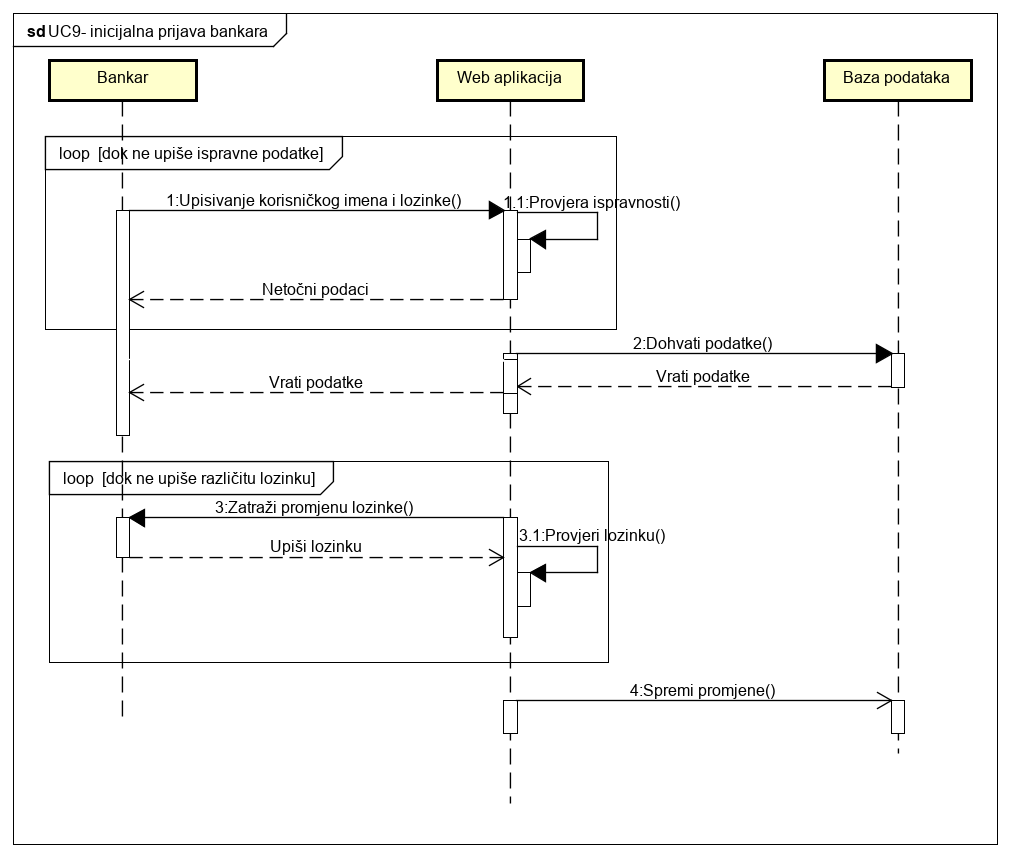
\includegraphics[scale=0.6]{slike/UC9- inicijalna prijava bankara.PNG}
					\centering
					\caption{Sekvencijski dijagram za UC9}
					\label{fig:uc9}
				\end{figure}
			\eject
			
			\noindent{\textbf{UC17 -  Ugovranje debitne kartice }}
			
			Klijent šalje zahtjev za ugovaranje debitne kartice. Bankar upisuje klijentov OIB dok ne upiše ispravan jedanaestero znamenkasti broj, a poslužitelj provjerava ispravnost tog OIB-a. Poslužitelj dohvaća podatke o klijentu iz baze podataka i prikazuje ih bankaru. Bankar odabire opciju „Dodaj debitnu karticu“ kako bi ispunio klijentov zahtjev. Sustav dodaje debitnu karticu i sprema promjene u bazu podataka. Nakon toga, klijentu se omogućava uvid u broj kartice i račun uz koji je kartica vezana.
			\eject
			
			\begin{figure}[H]
				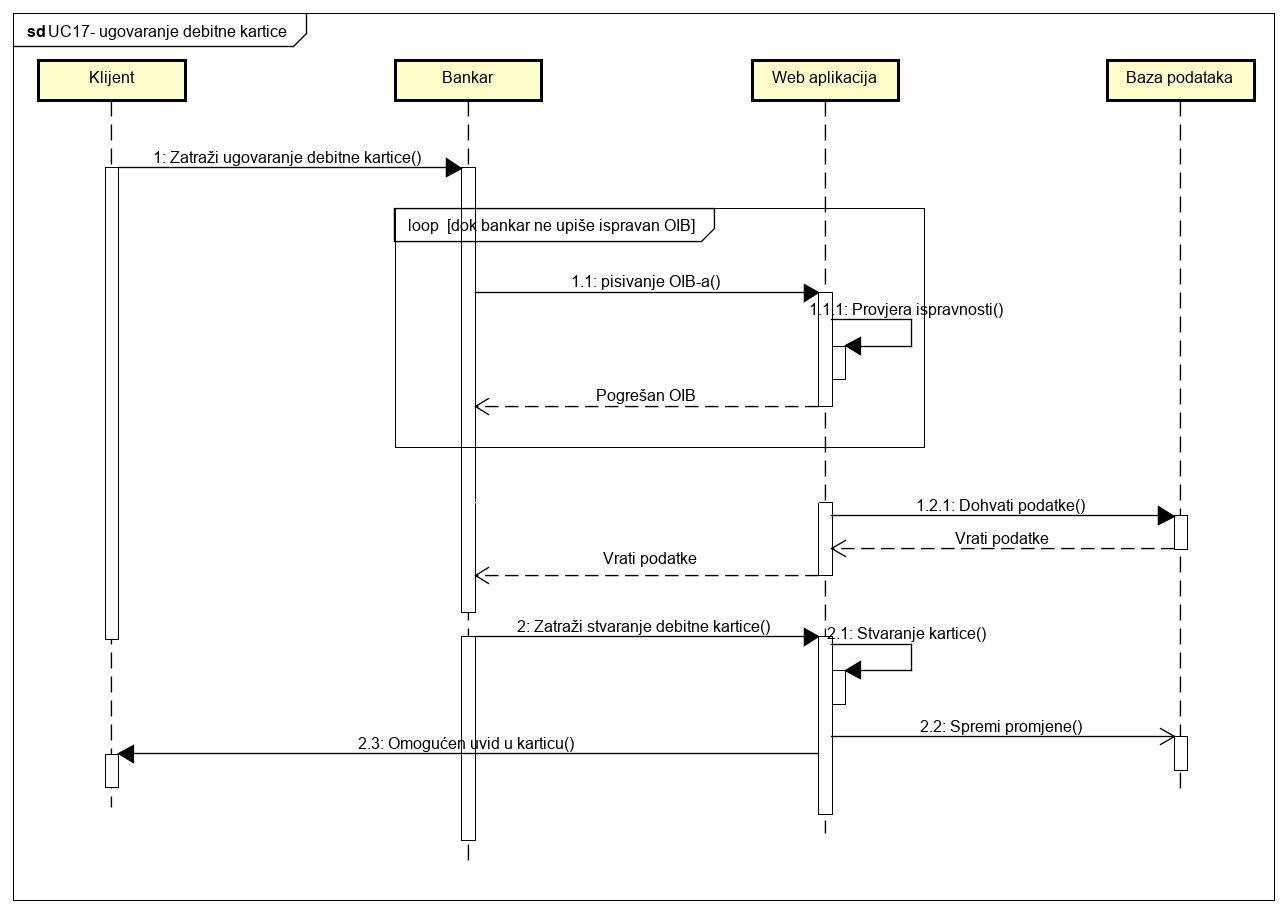
\includegraphics[scale=0.5]{slike/UC17- ugovaranje debitne kartice.PNG}
				\centering
				\caption{Sekvencijski dijagram za UC17}
				\label{fig:uc17}
			\end{figure}
			\eject
			
			\noindent{\textbf{UC21 -  Ugovaranje kredita}}
			
			
			Budući da klijent želi ugovoriti kredit, bankar prvo upisuje OIB klijenta kako bi sustav dohvatio njegove podatke. Bankar upisuje OIB dok sustav ne potvrdi ispravnost. Sustav zatraži od baze podataka klijentove podatke i prikazuje ih bankaru na uvid. Bankar šalje zahtjev za ugovaranjem kredita. Sustav traži potrebne podatke koje onda bankar upisuje. Sve promjene spremaju se u bazu podataka, a klijentov zahtjev za odabir kredita sustav šalje službeniku za odobravanje kredita.
			\eject
			
			\begin{figure}[H]
				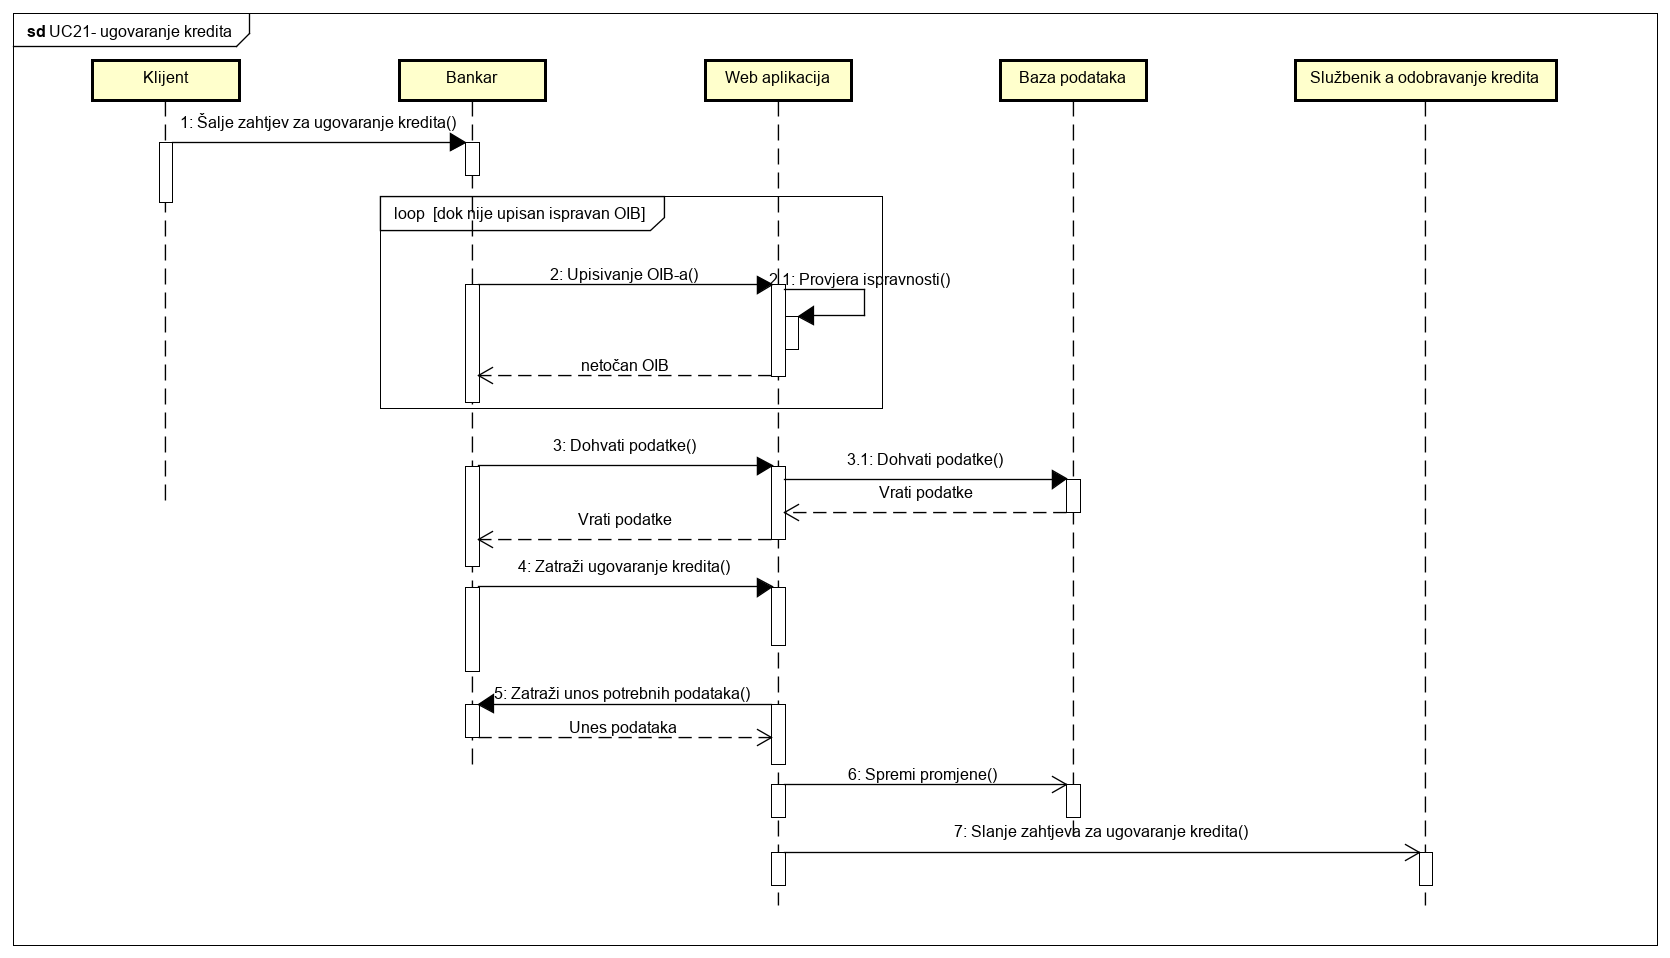
\includegraphics[scale=0.43]{slike/UC21- ugovaranje kredita.PNG}
				\centering
				\caption{Sekvencijski dijagram za UC21}
				\label{fig:uc21}
			\end{figure}
			\eject
			
			\noindent{\textbf{UC33 -  Registracija korisnika}}
			
			
			Ukoliko se korisnik želi registrirati, u aplikaciju upisuje svoj OIB i privremeni ključ koji je dobio od bankara. Poslužitelj provjerava ispravnost upisanih podataka. Ukoliko su uneseni podaci netočni, sustav ispisuje poruku o netočnim podacima i izlazi iz sustava. Ako su podaci ispravni, sustav traži od korisnika unos novog korisničkog imena i lozinke. Poslužitelj dohvaća podatke o klijentu iz baze podataka. Klijent upisuje novo korisničko ime i lozinku, a poslužitelj provjerava dostupnost korisničkog imena. Klijent upisuje novo koirsničko ime dok se ne razlikuje od ostalih spremljenih korisničkih imena ostalih klijenata. Nakon toga, klijent je uspješno registriran u sustav, a poslužitelj sprema promjene u bazu podataka.
			\eject
			
			\begin{figure}[H]
				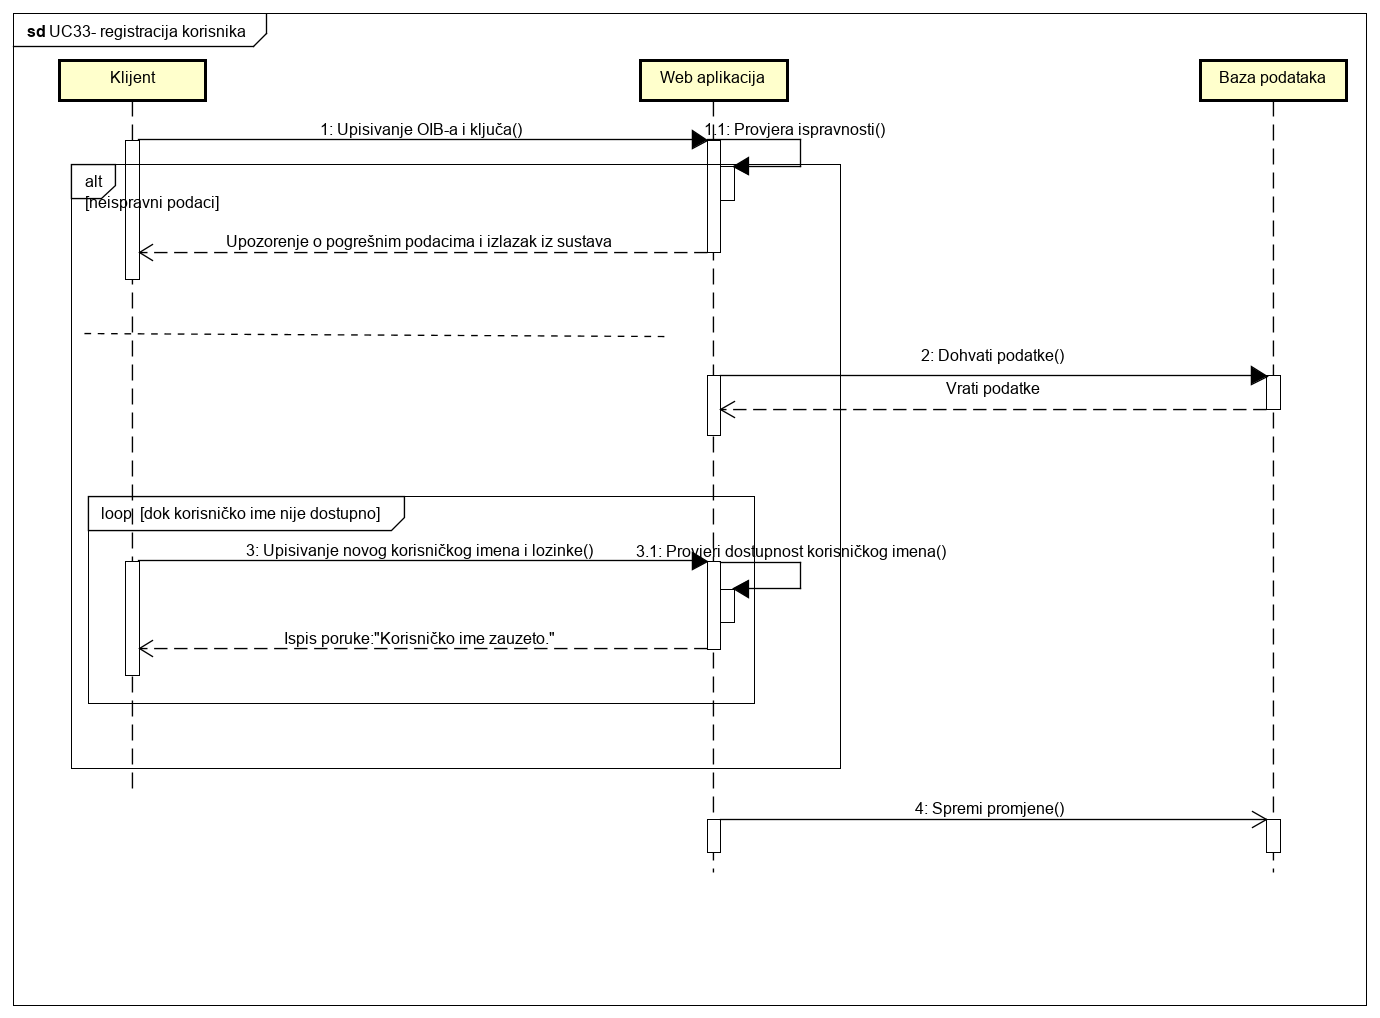
\includegraphics[scale=0.50]{slike/UC33- registracija korisnika.PNG}
				\centering
				\caption{Sekvencijski dijagram za UC33}
				\label{fig:uc33}
			\end{figure}
			\eject
			
	
		\section{Ostali zahtjevi}
			 
			 \begin{packed_item}
			 	\item Sustav mora podržavati rad više korisnika u stvarnom vremenu
			 	\item Aplikacija mora podržavati hrvatsku abecedu (dijakritičke znakove)
			 	\item Izvršavanje dijela programa u kojem se pristupa bazi podataka ne smije 
			 	trajati duže od nekoliko sekundi 
			 	\item Veza s bazom podataka mora biti kvalitetno zaštićena, brza i otporna na vanjske
			 	greške
			 	\item Nepravilno korištenje korisničkog sučelja ne smije narušiti funkcionalnost
			 	i rad sustava	
			 	\item Sustav treba biti jednostavan za upotrebu kako bi ga korisnici mogli koristiti
			 	bez opširnih uputa
			 	\item Nadogradnja sustava ne smije narušavati postojeće funkcionalnosti sustava
			 	\item Korisnički podaci jednog klijenta ne smiju biti vidljivi ostalim klijentima
			 	\item Klijent ne može mijenjati osobne podatke svog profila niti podatke o računima
			 	i karticama
			 	\item Svi računi moraju imati sliku profila
			 	\item Kao valuta se koristi HRK
			 	\item Svaki tekući račun treba imati dozvoljeno prekoračenje, a svaka kreditna kartica ugovoren limit.
			 	\item Jednom mjesečno korisnik treba dobiti izvod po svim transakcijskim
			 	računima i kreditnim karticama u PDF i XLS obliku
			 \end{packed_item}
